\documentclass[11pt]{article}

\usepackage[T1]{fontenc}
\usepackage[utf8]{inputenc}
\usepackage{lmodern}
\usepackage[margin=1in]{geometry}
\usepackage{graphicx}
\usepackage{booktabs}
\usepackage{longtable}
\usepackage{array}
\usepackage{caption}
\usepackage{hyperref}
\usepackage{microtype}

\setlength{\emergencystretch}{2em}

\hypersetup{
  colorlinks=true,
  linkcolor=black,
  citecolor=black,
  urlcolor=blue
}

\newcommand{\braindough}{\textsc{Braindough}}
\newcommand{\boldfive}{BOLD5000}
\newcommand{\rsq}{$R^2$}

\title{\braindough: A Local-First Neuroencoding Harness with a \boldfive{} Metadata-Control Benchmark}
\author{Peyton Kadej}
\date{2026-05-09}

\begin{document}
\maketitle

\begin{abstract}
Large public visual fMRI datasets make it practical to test neuroencoding
workflows against measured brain data before investing in heavyweight model
features or bespoke stimulus pipelines. This preprint describes a local-first
extension of \braindough{} for \boldfive{} Release 1.0 and reports the most
informative current result: a small source-family metadata signal that recurs
across subjects, ROIs, timing runs, and split variants. The benchmark uses ridge
regression on coarse stimulus provenance features, not image pixels or deep
neural features, and is therefore intended as a metadata-control,
provenance-content baseline, and harness-validation task rather than as a
competitive neural encoding model. Across four \boldfive{} participants and six
visual ROIs, the primary source-family rows produced mean Pearson $r=0.0748$
and mean \rsq{} $=0.00244$, with the strongest effects in PPA and LOC rather
than early visual cortex. In the full TR34 run, the best source-family row was
CSI2 LHPPA ($r=0.154$, \rsq{} $=0.0161$), with a run-level max-statistic
permutation $p=0.000999$ over the searched subject, ROI, and model grid. The
canonical primary summary uses TR34 for CSI1--CSI3 and TR3 for CSI4. A
grouped-filename sensitivity analysis eliminated exact repeated-filename
train/validation crossings and retained a positive best source-family result
(CSI2 LHPPA, $r=0.175$, \rsq{} $=0.0317$, max-statistic $p=0.00990$ with 100
permutations). These results support \braindough{} as a reproducible
measured-data evaluation harness and establish a concrete metadata baseline that
future image-feature encoders can be evaluated against.
\end{abstract}

\section{Introduction}

The \boldfive{} dataset is a slow event-related fMRI study designed around
large-scale natural image stimuli drawn from standard computer-vision image
sources including SUN, COCO, and ImageNet \cite{chang2019bold5000}. This makes
it useful not only for modeling visual cortex, but also for testing whether an
analysis system can ingest real measured neuroimaging data, preserve dataset
provenance, and report statistical checks before scaling to more expressive
models.

\braindough{} is a local-first experimental harness for brain-modeling
experiments. Its design goal is practical reproducibility on a workstation: the
repository contains code, tests, configs, and lightweight reports, while large
datasets, model weights, caches, and run outputs live outside the checkout under
a user-configured \texttt{BRAINDOUGH\_HOME}. The current implementation includes
fake backends for CI and measured-data adapters for \boldfive{} Release 1.0 ROI
data.

The most interesting current result is intentionally modest. Coarse
source-family metadata yields small positive validation correlations and low,
sometimes near-zero, validation \rsq{} values, especially in LOC and PPA. This
should not be read as evidence that visual
cortex ``encodes filenames'' or that source-family metadata is a good encoding
model. Instead, it is a useful baseline: if a future image-feature model cannot
beat this source/provenance-content control under the same split, it is not yet
demonstrating much beyond broad image-source structure.

\section{Dataset and Task}

The benchmark uses \boldfive{} Release 1.0 processed ROI vectors and trial
metadata. Release 1.0 is useful for a light, local benchmark because the
processed ROI matrices are straightforward to run without reproducing the full
fMRI preprocessing pipeline. The adapter records the release label, provenance,
dataset terms, and a source caveat in each run manifest. The manuscript does
not vendor raw \boldfive{} data or stimulus images.

Each run selects 1024 trials per subject using a fixed random seed
(20260509). TR34 denotes the Release 1.0 combined TR3/TR4 ROI timing file. The
primary timing is TR34 for CSI1--CSI3. CSI4 is reported from TR3 in the
canonical primary summary because the \boldfive{} guidance recommends TR3 for
CSI4 \cite{bold5000repo}; TR34 for CSI4 is retained only as timing sensitivity.
All subjects use the same six ROI labels: left and right early visual cortex
(LHEarlyVis, RHEarlyVis), LOC (LHLOC, RHLOC), and PPA (LHPPA, RHPPA).

Because \boldfive{} Release 2.0 provides updated functional estimates, including
optimized GLM outputs, this Release 1.0 ROI benchmark should be interpreted as a
local harness-validation and metadata-baseline analysis rather than as the
definitive \boldfive{} encoding benchmark \cite{bold5000repo}.

Three metadata models are evaluated per subject and ROI:

\begin{itemize}
  \item \texttt{source\_family}: one-hot stimulus source-family indicators
  plus a repeated-stimulus flag (four features in the Release 1.0 adapter);
  \item \texttt{token\_hash}: hashed filename-token features used only as a
  leakage-stress diagnostic;
  \item \texttt{source\_plus\_token\_hash}: concatenation of the two feature
  blocks, also diagnostic.
\end{itemize}

The primary scientific interpretation is restricted to \texttt{source\_family}.
Filename-token rows are reported by the harness so that repeated-stimulus and
identifier effects are visible during development, but they are not treated as
scientific encoding claims.

\section{Methods}

For each subject, ROI, and model family, the backend fits ridge regression
\cite{hoerl1970ridge} on a 75/25 split. Ridge alpha is selected from
$\{0.1, 1, 10, 100\}$ by validation Pearson correlation. The same
alpha-selection rule is replayed inside the row-wise and max-statistic
permutation procedures. Because alpha is selected on the validation split, all
scores are described as validation benchmark scores rather than as independent
test estimates.

The default primary split stratifies by source family. A separate
grouped-filename split stratifies by source while assigning exact repeated
filenames to only one side of the train/validation boundary. This grouped split
is used as a leakage-control sensitivity, not as a replacement for a full
image-identity generalization study.

Model quality is reported as validation Pearson correlation and validation
\rsq{}. Pearson $r$ and \rsq{} are interpreted separately: small positive
correlations can be detectable while \rsq{} remains near zero or negative.
\rsq{} is therefore treated as the practical predictive-performance metric and
Pearson $r$ as a directional association metric. Bootstrap intervals are
computed by resampling validation trials. Within-row permutation values are
uncorrected diagnostics. Max-statistic values are reported separately at the run
level. Both use the largest positive Pearson statistic and are therefore
one-sided diagnostics for positive predictive association. Permutation
$p$-values use the finite-sample $(b+1)/(n+1)$ convention so that
random-permutation $p$-values are never zero \cite{phipson2010permutation}.

The code changes required for this benchmark are small and auditable: seeded
random trial selection, subject/ROI-aware Release 1.0 indexing, split-balance
diagnostics, repeated-filename leakage diagnostics, max-statistic permutations,
and a repo-local Tectonic build target for this manuscript.

\section{Results}

\subsection{Primary source-family benchmark}

Table~\ref{tab:area-summary} summarizes the canonical primary result:
CSI1--CSI3 use TR34, and CSI4 uses TR3. Across the 24 source-family rows,
mean Pearson $r$ is 0.0748, mean \rsq{} is 0.00244, and 14 of 24 rows have
validation \rsq{} $>0$. The effect is spatially structured: PPA has the
largest average source-family score, followed by LOC, while early visual ROIs
remain near zero by \rsq{}.

\begin{table}[ht]
  \centering
  \caption{Primary source-family results by ROI family. CSI1--CSI3 use TR34 and CSI4 uses TR3. Full row-level values are committed in \texttt{tables/primary\_source\_family\_results.csv}.}
  \label{tab:area-summary}
  \begin{tabular}{lrrrr}
    \toprule
    Summary group & $n$ & Mean $r$ & Mean \rsq{} & Rows with \rsq{} $>0$ \\
    \midrule
    All primary rows & 24 & 0.0748 & 0.00244 & 14 \\
    Early visual ROIs & 8 & 0.0281 & -0.00566 & 0 \\
    LOC ROIs & 8 & 0.0760 & 0.00294 & 7 \\
    PPA ROIs & 8 & 0.1204 & 0.01005 & 7 \\
    \bottomrule
  \end{tabular}
\end{table}

The best result in the primary TR34 all-subject run is CSI2 LHPPA under the
source-family model ($r=0.154$, \rsq{} $=0.0161$, bootstrap interval
$[0.111, 0.199]$). The max-statistic permutation value for the best observed
TR34 grid result is $p=0.000999$ with 1000 permutations. For CSI4 at TR3, the
best source-family row is LHPPA ($r=0.0820$, \rsq{} $=0.00210$), and the full
TR3 run also has a run-level max-statistic $p=0.000999$. For both
1000-permutation runs, $p=0.000999$ is the minimum finite value under the
$(b+1)/(n+1)$ estimator. These values are detectable, but the practical effect
sizes are small.

\begin{figure}[ht]
  \centering
  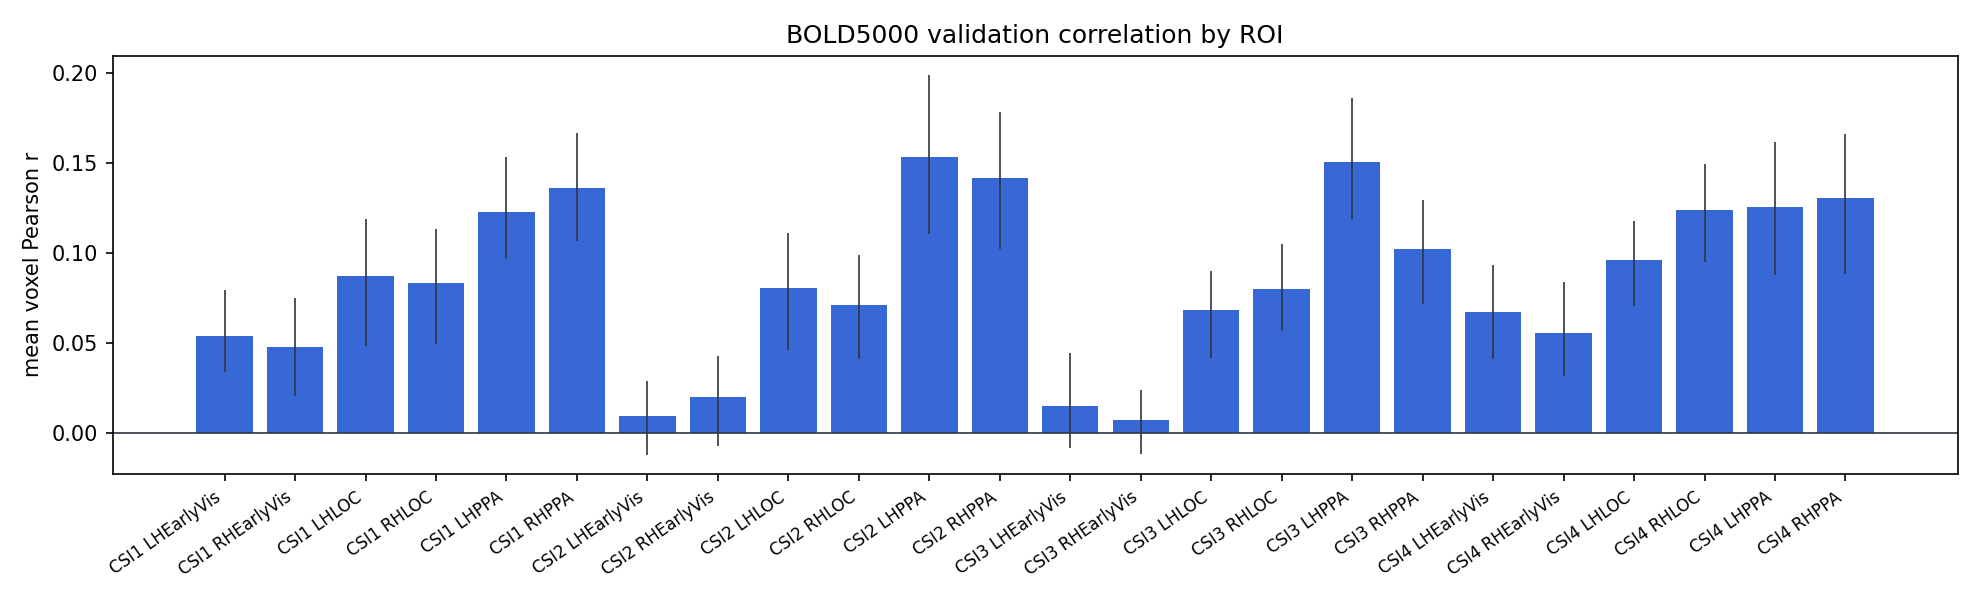
\includegraphics[width=0.96\linewidth]{figures/tr34_roi_scores.png}
  \caption{TR34 source-family and diagnostic model scores across subjects and ROIs. TR34 is the primary timing for CSI1--CSI3.}
  \label{fig:tr34-roi}
\end{figure}

\begin{figure}[ht]
  \centering
  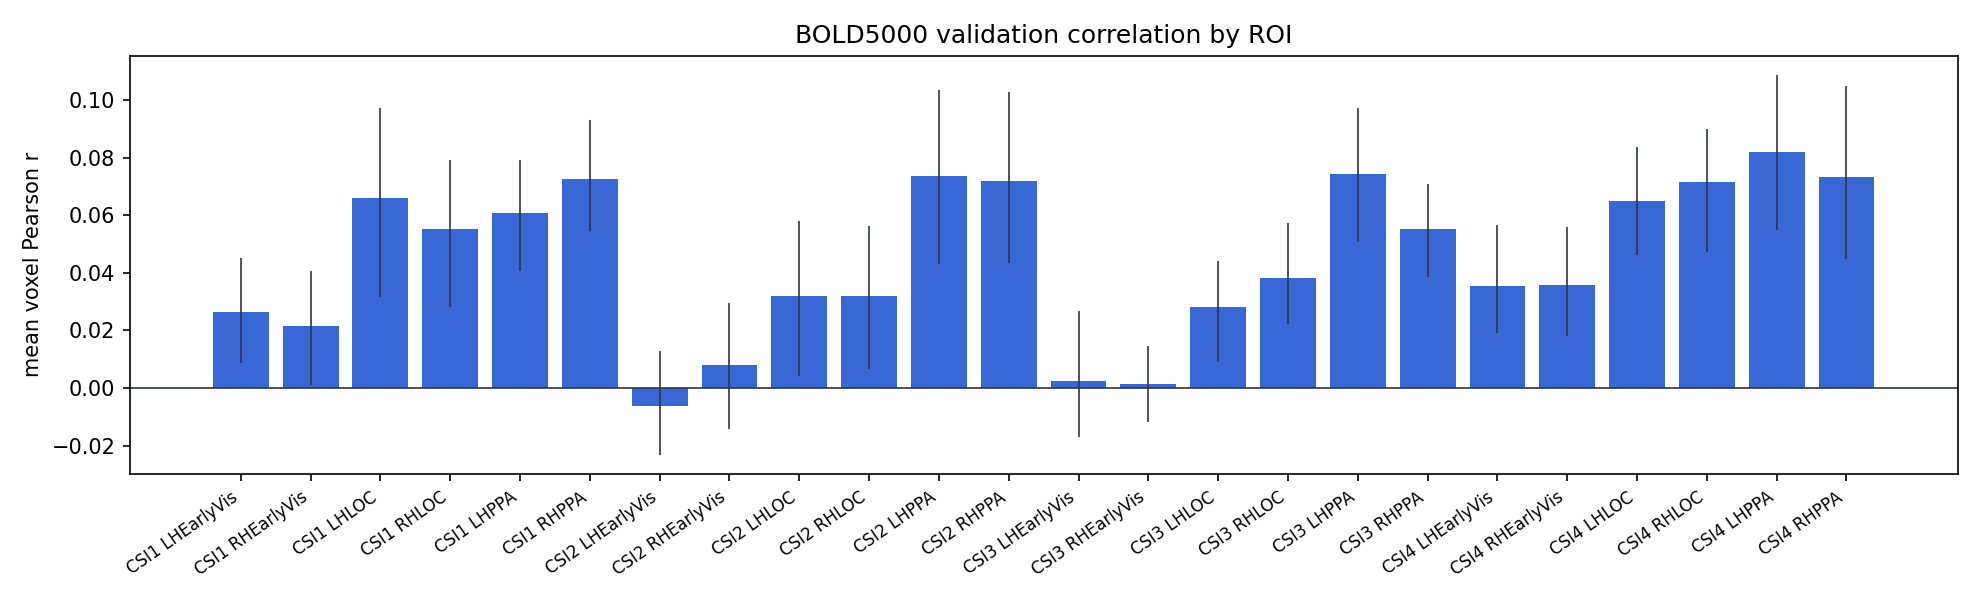
\includegraphics[width=0.96\linewidth]{figures/tr3_roi_scores.png}
  \caption{TR3 timing sensitivity. CSI4 TR3 rows are used in the canonical primary summary.}
  \label{fig:tr3-roi}
\end{figure}

\subsection{Repeated-filename sensitivity}

The primary source-stratified split can allow exact filenames that occur more
than once in the selected trials to appear on both sides of the train/validation
boundary. This is not, by itself, evidence that the source-family model is
leaking image identity: source family is a coarse provenance feature and does
not include filename identity. It is nevertheless a useful stress point for a
benchmark harness.

The grouped-filename sensitivity sets exact repeated-filename crossings to
zero for every subject. The strongest source-family row remains CSI2 LHPPA
($r=0.175$, \rsq{} $=0.0317$, bootstrap interval $[0.123, 0.216]$), with a
max-statistic value of $p=0.00990$. Because this sensitivity used only 100
permutations, $p=0.00990$ is the minimum finite value possible under the
reported estimator and should be interpreted as zero exceedances among 100
shuffled max statistics rather than as a precisely estimated $p$-value. Across
all 24 source-family rows in the grouped sensitivity, mean Pearson $r$ is
0.0809 and mean \rsq{} is 0.00559.

The grouped split controls exact repeated-filename train/validation crossings;
it does not eliminate broader source-, category-, session-, or
image-distribution differences. Train/validation source-family counts and
repeated-filename crossing counts are committed under \texttt{tables/} in the
TR34 split-balance, TR34 leakage-diagnostic, grouped-TR34 split-balance, and
grouped-TR34 leakage-diagnostic CSV files.

\begin{figure}[ht]
  \centering
  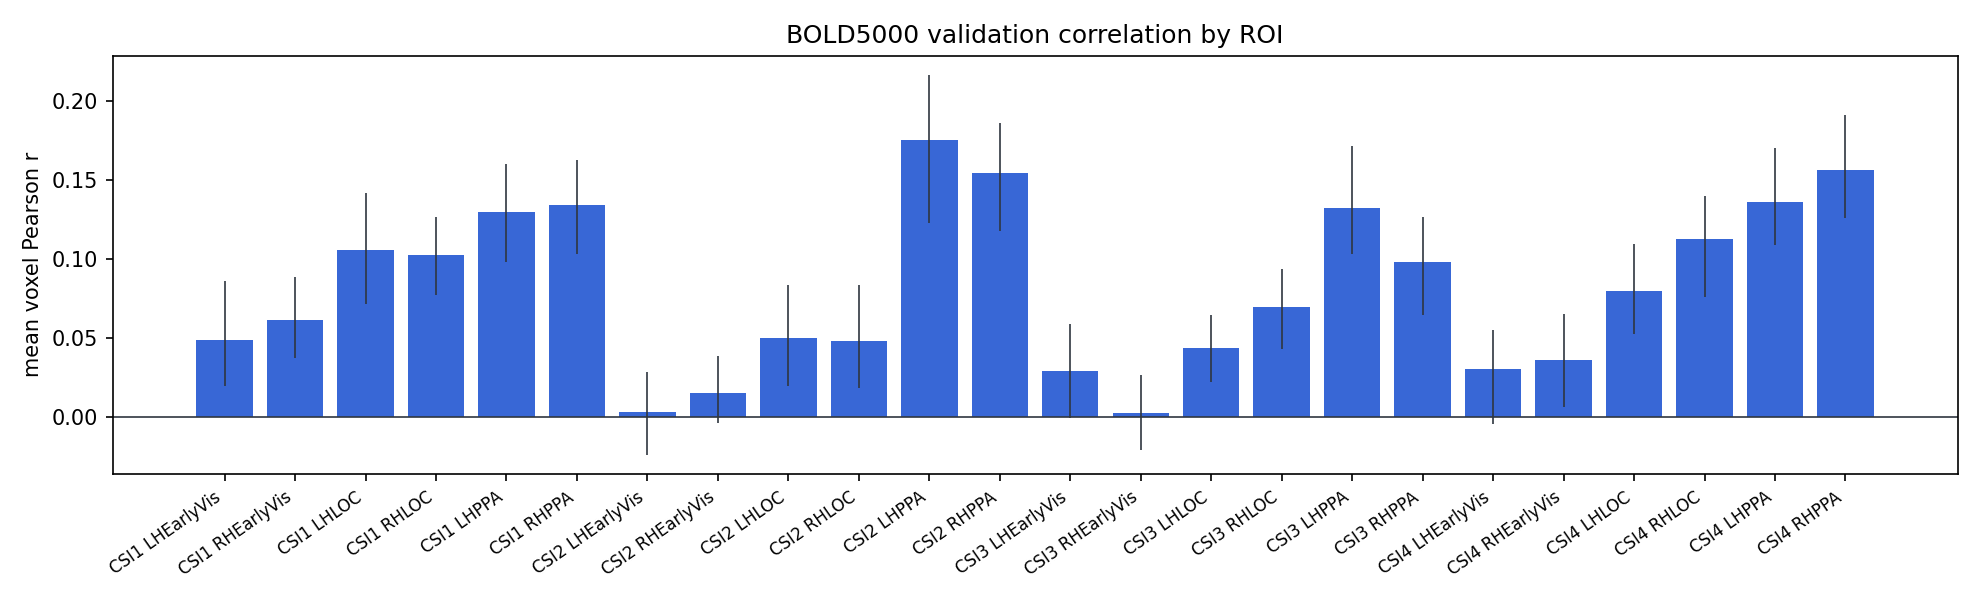
\includegraphics[width=0.96\linewidth]{figures/grouped_tr34_roi_scores.png}
  \caption{TR34 grouped-filename sensitivity. Exact repeated-filename train/validation crossings are eliminated while preserving the small source-family signal.}
  \label{fig:grouped-roi}
\end{figure}

\section{Discussion}

The result is best interpreted as a measured-data harness check with scientific
guardrails. The source-family signal recurs across subjects, ROIs, timing runs,
and split variants, is strongest in high-level visual ROIs, and remains positive
after a grouped-filename split that removes exact repeated-filename
train/validation crossings. The same evidence also constrains the claim:
explained variance is tiny, source-family labels are coarse, and the current
adapter uses Release 1.0 ROI vectors rather than pixel-level image features,
captions, model embeddings, voxelwise encoding, or Release 2.0 GLM outputs.

This makes the result useful precisely because it is limited. It establishes a
low but measurable benchmark bar for future \braindough{} encoders. A model
using CLIP features, caption features, low-level image statistics, or learned
visual embeddings should be expected to exceed this metadata baseline if it
captures image-level information beyond source-family structure under the same
subject, ROI, trial, and split diagnostics. If it does not, the benchmark can
catch that failure early.

\section{Limitations}

Several limitations are deliberate. First, this is not a state-of-the-art
\boldfive{} analysis and does not estimate noise ceilings. Because \boldfive{}
Release 2.0 provides updated functional estimates, including optimized GLM
outputs, the Release 1.0 ROI benchmark here is a local harness-validation and
metadata-baseline analysis rather than the definitive \boldfive{} encoding
benchmark \cite{bold5000repo}. Second, the benchmark uses 1024 selected trials per subject rather
than the full release. Third, the grouped-filename sensitivity controls exact
repeated filenames but does not replace stronger image-identity, session, or
category-generalization splits. Fourth, source-family labels may proxy broad
visual and semantic differences among SUN, COCO, ImageNet, and other source
groups; this is why the result is described as a provenance-content baseline
rather than a mechanistic neural code. Fifth, the grouped sensitivity used 100
permutations for local runtime reasons, so its max-statistic value has coarse
finite resolution. Sixth, permutation and bootstrap summaries are conditional
on the selected \boldfive{} Release 1.0 trials and subjects. They are not
population-level inference over human participants. Bootstrap intervals are
validation-trial resampling intervals, not subject-level confidence intervals
and not selection-adjusted intervals.

\section{Reproducibility}

The committed configs live in \path{experiments/local/} and are named for the
TR34, TR3, and grouped-TR34 sensitivity runs.

The corresponding root commands are the three \texttt{run-bold5000-preprint-*}
targets in the root \texttt{justfile}. Routine repository validation runs
through \texttt{just ci}. This PDF is built with the \texttt{preprint-build}
target against this timestamped directory.

\section{Acknowledgments and AI Assistance}

\boldfive{} was produced and released by Chang and colleagues
\cite{chang2019bold5000}. ChatGPT 5.5 Extended Pro was used for iterative
scientific critique, claim scoping, and drafting assistance. All numerical
results reported here come from committed \braindough{} configs and run
artifacts, not from model-generated estimates.

\appendix

\section{Run Summary}

\begin{table}[ht]
  \centering
  \caption{Run-level summary. Full run IDs and notes are committed in \texttt{tables/run\_summary.csv}.}
  \label{tab:run-summary}
  \begin{tabular}{llrrrr}
    \toprule
    Run & Split & Perms & Best ROI & Best $r$ & Max-stat $p$ \\
    \midrule
    TR34 primary & stratified source & 1000 & CSI2 LHPPA & 0.154 & 0.000999 \\
    TR3 timing & stratified source & 1000 & CSI4 LHPPA & 0.082 & 0.000999 \\
    TR34 grouped sensitivity & grouped filename & 100 & CSI2 LHPPA & 0.175 & 0.00990 \\
    \bottomrule
  \end{tabular}
\end{table}

\section{Canonical Primary Source-Family Rows}

\footnotesize
\begin{longtable}{lllrrrr}
\caption{Canonical primary source-family rows. CSI1--CSI3 use TR34 and CSI4 uses TR3. Within-row $p$ values are uncorrected diagnostics.}\label{tab:primary-rows}\\
\toprule
Subject & TR & ROI & $r$ & \rsq{} & Within-row $p$ & Bootstrap interval \\
\midrule
\endfirsthead
\toprule
Subject & TR & ROI & $r$ & \rsq{} & Within-row $p$ & Bootstrap interval \\
\midrule
\endhead
CSI1 & TR34 & LHEarlyVis & 0.054 & -0.0006 & 0.000999 & [0.034, 0.079] \\
CSI1 & TR34 & RHEarlyVis & 0.048 & -0.0028 & 0.000999 & [0.020, 0.075] \\
CSI1 & TR34 & LHLOC & 0.087 & 0.0041 & 0.000999 & [0.048, 0.119] \\
CSI1 & TR34 & RHLOC & 0.084 & 0.0057 & 0.000999 & [0.050, 0.114] \\
CSI1 & TR34 & LHPPA & 0.123 & 0.0109 & 0.000999 & [0.097, 0.153] \\
CSI1 & TR34 & RHPPA & 0.136 & 0.0149 & 0.000999 & [0.107, 0.167] \\
CSI2 & TR34 & LHEarlyVis & 0.010 & -0.0074 & 0.168831 & [-0.012, 0.029] \\
CSI2 & TR34 & RHEarlyVis & 0.020 & -0.0058 & 0.001998 & [-0.007, 0.043] \\
CSI2 & TR34 & LHLOC & 0.081 & 0.0027 & 0.000999 & [0.046, 0.111] \\
CSI2 & TR34 & RHLOC & 0.071 & 0.0025 & 0.000999 & [0.041, 0.099] \\
CSI2 & TR34 & LHPPA & 0.154 & 0.0161 & 0.000999 & [0.111, 0.199] \\
CSI2 & TR34 & RHPPA & 0.142 & 0.0148 & 0.000999 & [0.103, 0.179] \\
CSI3 & TR34 & LHEarlyVis & 0.015 & -0.0096 & 0.041958 & [-0.008, 0.044] \\
CSI3 & TR34 & RHEarlyVis & 0.006 & -0.0079 & 0.255744 & [-0.013, 0.024] \\
CSI3 & TR34 & LHLOC & 0.069 & 0.0037 & 0.000999 & [0.042, 0.090] \\
CSI3 & TR34 & RHLOC & 0.080 & 0.0048 & 0.000999 & [0.057, 0.105] \\
CSI3 & TR34 & LHPPA & 0.151 & 0.0161 & 0.000999 & [0.119, 0.187] \\
CSI3 & TR34 & RHPPA & 0.102 & 0.0067 & 0.000999 & [0.072, 0.130] \\
CSI4 & TR3 & LHEarlyVis & 0.036 & -0.0046 & 0.024975 & [0.019, 0.056] \\
CSI4 & TR3 & RHEarlyVis & 0.036 & -0.0067 & 0.003996 & [0.018, 0.056] \\
CSI4 & TR3 & LHLOC & 0.065 & -0.0003 & 0.000999 & [0.046, 0.084] \\
CSI4 & TR3 & RHLOC & 0.071 & 0.0002 & 0.000999 & [0.047, 0.090] \\
CSI4 & TR3 & LHPPA & 0.082 & 0.0021 & 0.000999 & [0.055, 0.109] \\
CSI4 & TR3 & RHPPA & 0.073 & -0.0014 & 0.000999 & [0.045, 0.105] \\
\bottomrule
\end{longtable}
\normalsize

\begin{thebibliography}{9}

\bibitem{chang2019bold5000}
Chang, N., Pyles, J. A., Marcus, A., Gupta, A., Tarr, M. J., and Aminoff,
E. M. \boldfive{}, a public fMRI dataset while viewing 5000 visual images.
\emph{Scientific Data} 6, 49 (2019). doi:10.1038/s41597-019-0052-3.

\bibitem{bold5000dataset}
Chang, N. et al. \boldfive{}. figshare (2019).
\url{https://doi.org/10.1184/R1/6459449.v4}.

\bibitem{bold5000repo}
BOLD5000-dataset. Official code release for \boldfive{} Release 2.0.
\url{https://github.com/BOLD5000-dataset/BOLD5000}.

\bibitem{hoerl1970ridge}
Hoerl, A. E. and Kennard, R. W. Ridge regression: biased estimation for
nonorthogonal problems. \emph{Technometrics} 12(1), 55--67 (1970).

\bibitem{phipson2010permutation}
Phipson, B. and Smyth, G. K. Permutation p-values should never be zero:
calculating exact p-values when permutations are randomly drawn.
\emph{Statistical Applications in Genetics and Molecular Biology} 9(1), Article
39 (2010). doi:10.2202/1544-6115.1585.

\end{thebibliography}

\end{document}
